
%%******************************************************************************
%% SECTION - Data 
%%******************************************************************************

\subsection{Dados}
\subsubsection{Variação de Tensão}
\begin{table}[h!]
	\begin{tabular}{r l|l p{12cm} }
		\textcolor{black}{Voltagem} &&& 	{Contato metálico}\\
		\textcolor{gray}{$12V$} &&& 				{OK}\\
		\textcolor{gray}{$21V$} &&& 				{OK}\\
 	\end{tabular}
\end{table}

\subsubsection{Alcance fora d'água}
\begin{table}[h!]
	\begin{tabular}{r l|l p{12cm} }
		\textcolor{black}{Distância} &&& 	{Contato metálico}\\
		\textcolor{gray}{1cm} &&& 				{OK}\\
		\textcolor{gray}{2cm} &&& 				{OK}\\
		\textcolor{gray}{3cm} &&& 				{OK}\\
		\textcolor{gray}{3.5cm} &&& 				{Não}\\
 	\end{tabular}
\end{table}

\begin{figure}[h!]
 \centering
 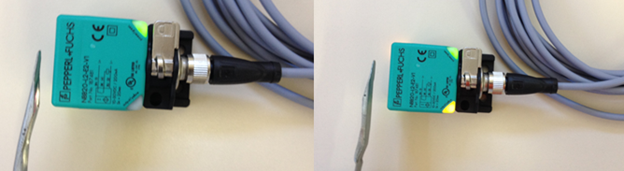
\includegraphics[width=1\columnwidth]{indutivo/figs/indutivo_alcance.png}
 \caption{Alcance do sensor indutivo fora d'água}
 \label{fig:indu_alc}
 \end{figure}
 
 \subsubsection{Alcance dentro d'água}
 \begin{table}[H]
	\begin{tabular}{r l|l p{12cm} }
		\textcolor{black}{Distância} &&& 	{Contato metálico}\\
		\textcolor{gray}{1cm} &&& 				{OK}\\
		\textcolor{gray}{2cm} &&& 				{OK}\\
		\textcolor{gray}{3cm} &&& 				{OK}\\
		\textcolor{gray}{3.5cm} &&& 				{Não}\\
 	\end{tabular}
\end{table}

\begin{figure}[H]
 \centering
 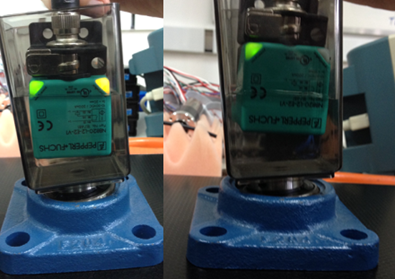
\includegraphics[width=1\columnwidth]{indutivo/figs/indutivo_agua.png}
 \caption{Alcance do sensor indutivo dentro d'água}
 \label{fig:indu_agu}
 \end{figure}
 
 \subsubsection{Aproximação não faceada}
  \begin{table}[h!]
	\begin{tabular}{r l|l p{12cm} }
		\textcolor{black}{Aproximação} &&& 	{Contato metálico}\\
		\textcolor{gray}{Faceada} &&& 				{OK}\\
		\textcolor{gray}{Não faceada} &&& 				{Não}\\
 	\end{tabular}
\end{table}

\begin{figure}[h!]
 \centering
 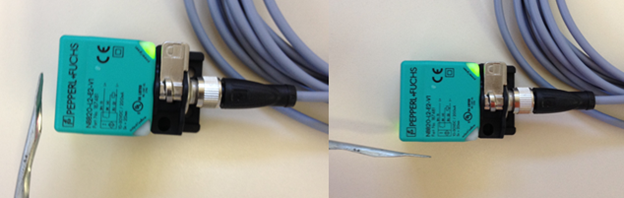
\includegraphics[width=1\columnwidth]{indutivo/figs/indutivo_faceado.png}
 \caption{Aproximação faceada e não faceada.}
 \label{fig:indu_fac}
 \end{figure}
 
 \subsubsection{Teste de comunicação via LAN}
   \begin{table}[H]
	\begin{tabular}{r l|l p{12cm} }
		\textcolor{black}{Aproximação} &&& 	{Booleano}\\
		\textcolor{gray}{Presença de objeto metálico} &&& 				{True}\\
		\textcolor{gray}{Ausência de objeto metálico} &&& 				{False}\\
 	\end{tabular}
\end{table}
 
 
\label{dados}




  